% !TeX root = ../../../thesis.tex

\subsection{Gold Sequences}
\label{subsec:gold-sequences}

Gold sequences are a type of PN sequence.
These codes are used for as C/A Code (Coarse Acquisition) in GPS satellites \cite{gold-in-sats}. 
They are created by using two LFS registers as shown in \autoref{fig:gold-lfsr}.
In this figure there are two vectors $s$ and $t$ and two polynomials $C$ and $D$.
For a sequence to be constructed in this way that is a Gold sequence, only preferred pairs of polynomials can be used \cite{kedia2012comparative}.
When we have the polynomials $p(x)$ and $q(x)$, which are a preferred pair and produce the PN sequences $d_1$ and $d_2$ respectively, the resulting set of Gold codes is defined as can be seen in \autoref{eq:gold-def}, where $T^n$ represent the cyclic shift of $n$ bits.

\begin{equation}
	\label{eq:gold-def}
	Gold(d_1, d_2) = \{ d_1, d_2, d_1 \oplus d_2, d_1 \oplus Td_2, d_1 \oplus T^2d_2, \dotsc, d_1 \oplus T^{L - 1}d_2 \}
\end{equation}


\begin{figure}[t]
	\centering
	\begin{tikzpicture}

		\node[block                  ] (last_register1) {$s_{n-1}$};
		\node[block, right = 1cm of last_register1] (second_last_register1) {$s_{n-2}$};
		\draw[line] (last_register1.east) -- (second_last_register1.west) ;

		\node[block, right = 3cm of second_last_register1] (second_register1) {$s_{1}$};
		\node[block, right = 1cm of second_register1] (mid_register1) {$s_{0}$};
		\draw[line] (second_register1.east) -- (mid_register1.west) ;

		\draw[dashed, line] (second_last_register1.east) -- (second_register1.west) ;

		\node[coordinate, right = 1cm of mid_register1] (output_point1) {};

		\node[XOR, scale=2, above = 2cm of second_register1] (first_xor1) {};
		\draw[line] (second_register1.north) -- (first_xor1.south) node [midway, right] {$C_1$};
		\draw[line] (mid_register1.north) |- (first_xor1.east) node [pos=0.21, right] {$C_0$};

		\node[coordinate, right = 1.5cm of second_last_register1] (h1) {};
		\node[XOR, scale=2, above = 2.5cm of h1] (mid_xor1) {};
		\draw[line] (first_xor1.west) -- (mid_xor1.east) ;
		\draw[dashed, line] (h1.north) -- (mid_xor1.south) ;

		\node[XOR, scale=2, above = 2cm of second_last_register1] (second_last_xor1) {};
		\node[XOR, scale=2, above = 2cm of last_register1] (last_xor1) {};

		\draw[line] (second_last_register1.north) -- (second_last_xor1.south) node [midway, right] {$C_{n-2}$};
		\draw[line] (mid_xor1.west) -- (second_last_xor1.east) ;
		
		\draw[line] (second_last_xor1.west) -- (last_xor1.east) ;
		\draw[line] (last_register1.north) -- (last_xor1.south) node [midway, right] {$C_{n-1}$};

		\node[coordinate, left = 1cm of last_register1] (return_point1) {};
		
		\draw[line] (last_xor1.west) -| (return_point1) -- (last_register1.west) ;

		%%%%%%%%%%%%%%%%%%%%%%%%%%%%%%%%%%%%%%%%%%%%%%%%%%%%%%%%%%%%%%%%%%%%%%%%%%%%


		\node[block, below = 2cm of last_register1] (last_register) {$t_{n-1}$};
		\node[block, right = 1cm of last_register] (second_last_register) {$t_{n-2}$};
		\draw[line] (last_register.east) -- (second_last_register.west) ;

		\node[block, right = 3cm of second_last_register] (second_register) {$t_{1}$};
		\node[block, right = 1cm of second_register] (mid_register) {$t_{0}$};
		\draw[line] (second_register.east) -- (mid_register.west) ;

		\draw[dashed, line] (second_last_register.east) -- (second_register.west) ;

		\node[coordinate, right = 1cm of mid_register] (output_point) {};

		\node[XOR, scale=2, below = 2cm of second_register] (first_xor) {};
		\draw[line] (second_register.south) -- (first_xor.north) node [midway, right] {$D_1$};
		\draw[line] (mid_register.south) |- (first_xor.east) node [pos=0.21, right] {$D_0$};

		\node[coordinate, right = 1.5cm of second_last_register] (h) {};
		\node[XOR, scale=2, below = 2.5cm of h] (mid_xor) {};
		\draw[line] (first_xor.west) -- (mid_xor.east) ;
		\draw[dashed, line] (h.south) -- (mid_xor.north) ;

		\node[XOR, scale=2, below = 2cm of second_last_register] (second_last_xor) {};
		\node[XOR, scale=2, below = 2cm of last_register] (last_xor) {};

		\draw[line] (second_last_register.south) -- (second_last_xor.north) node [midway, right] {$D_{n-2}$};
		\draw[line] (mid_xor.west) -- (second_last_xor.east) ;
		
		\draw[line] (second_last_xor.west) -- (last_xor.east) ;
		\draw[line] (last_register.south) -- (last_xor.north) node [midway, right] {$D_{n-1}$};

		\node[coordinate, left = 1cm of last_register] (return_point) {};
		
		\draw[line] (last_xor.west) -| (return_point) -- (last_register.west) ;

		%%%%%%%%%%%%%%%%%%%%%%%%%%%%%%%%%%%%%%%%%%%%%%%%%%%%%%%%%%%%%%%%

		\node[XOR, scale=2, below = 1cm of output_point1] (gold_xor) {};
		\draw[line] (mid_register1) -| (gold_xor) ;
		\draw[line] (mid_register) -| (gold_xor) ;
		\node[coordinate, right = 2cm of gold_xor] (gold_output) {} ;
		\draw[line] (gold_xor.east) -- (gold_output.west) node [midway, above] {output};


	\end{tikzpicture}
	\caption{Two linear feedback shifter registers of length $n$, with XOR gates to produce a set of Gold sequences.}
	\label{fig:gold-lfsr}
\end{figure}



\begin{figure}[tbp]
	\centering
	\includegraphics[width=0.9\textwidth]{chapters/cdma-chapters/codes/autocorr-gold.eps}
	\caption{Autocorrelation of one Gold sequence of length 1023.}
	\label{fig:autocorr-gold}
\end{figure}


\begin{figure}[tbp]
	\centering
	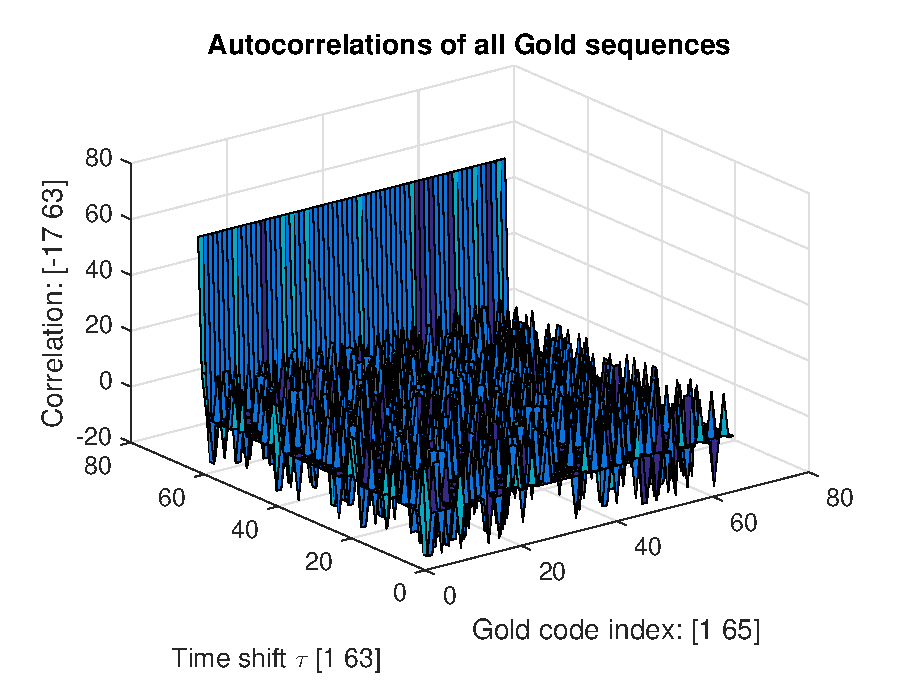
\includegraphics[width=0.9\textwidth]{chapters/cdma-chapters/codes/autocorr-gold-3d.eps}
	\caption{Autocorrelation of all Gold sequences in the same set of length 63.}
	\label{fig:autocorr-gold-3d}
\end{figure}




The autocorrelation properties of Gold sequences are not as good as that of the PN sequences, as can be seen from \autoref{fig:autocorr-gold}.
The autocorrelation of all the Gold sequences are plotted in \autoref{fig:autocorr-gold-3d} to illustrate the autocorrelation of all sequences look like each other.
Apart from the original two PN sequences the autocorrelation values are not two-valued, but are four-valued.
See \autoref{eq:autocorr-gold} and \autoref{eq:gold-t(n)} for the autocorrelation properties of Gold sequences.

\begin{equation}
	\label{eq:autocorr-gold}
	R(\tau) = 
		\begin{cases}
			L    							& \quad \text{if } \tau = 0 \\
			\{ -t(n), \ -1, \ t(n) - 2  \} 	& \quad \text{if } \tau \neq 0 \\
		\end{cases}
\end{equation}

\begin{equation}
	\label{eq:gold-t(n)}
	t(n) = 
		\begin{cases}
			1 + 2^{\frac{n+1}{2}} & \quad \text{for odd } n \\
			1 + 2^{\frac{n+2}{2}} & \quad \text{for even } n \\
		\end{cases}
\end{equation}

See \autoref{eq:corsscorr-gold} and \autoref{eq:gold-t(n)} for the cross-correlation properties of Gold sequences \cite{mitra2008pseudo}.

\begin{equation}
	\label{eq:corsscorr-gold}
	R_{xy}(\tau) = 	\{ -t(n), -1, t(n) - 2  \} 
\end{equation}


From these equations it is clear to see that the absolute maximum cross-correlation is bounded by $t(n)$.
See \autoref{tbl:gold-sequences-C-and-cross-corr} for the cross-correlation for different lengths of Gold sequences.


\begin{table}[tbp]
	\centering
	\begin{tabular}{  | l | l | l | }

		\hline
		Code Length (L)	& Number of Codes (C) 	& Peak cross-correlation ($|t(n)|$)	\\ \hline
		
		7				& 9						& 5						\\ \hline					
		31				& 33					& 9						\\ \hline			
		63				& 65					& 17					\\ \hline			
		127				& 129					& 17					\\ \hline	
		511				& 513					& 33					\\ \hline	
		1023			& 1025					& 65					\\ \hline	

	\end{tabular}
	\caption{Table showing the number of Gold sequences of the same length along with the peak cross-correlation. }
	\label{tbl:gold-sequences-C-and-cross-corr}

\end{table}

As seen from \autoref{tbl:gold-sequences-C-and-cross-corr} the scalability of the Gold sequences is good.
With a LFSR of length $n$, the sequence length is $L = 2^n - 1$ and the number of sequences is $C = 2^n + 1$.
Compared to the peak cross-correlation of the PN sequences, \autoref{tbl:pn-sequences-C-and-cross-corr}, the peak cross-correlation of the Gold sequences are lower for the same code length, see \autoref{tbl:gold-sequences-C-and-cross-corr}.



% Taken out because this is not used anywhere....

%When $n$ is chosen to be odd, something can be said about the approximate frequency of occurrence of the cross-correlation values, see \autoref{tbl:freq-occurence-gold-cross-correlation} \cite{holmes2007spread}.

%\begin{table}[h]
%	\centering
%	\begin{tabular}{ | l | l | }
%
%		\hline
%		$R_{xy}(\tau)$ 	& Frequency of occurrence	\\ \hline
%
%		$-1$			& 0.5					 	\\ \hline
%		$-t(n)$			& 0.25						\\ \hline
%		$t(n) - 2$		& 0.25						\\ \hline
%
%		
%
%	\end{tabular}
%	\caption{Table containing the approximate frequency of occurrence for all the cross-correlation values for $n$ odd.}
%	\label{tbl:freq-occurence-gold-cross-correlation}
%\end{table}



Not all Gold sequences have the balance property that the PN sequences do have.
Roughly half of the sequences in the same set are balanced, sometimes this can be as high as three quarters \cite{holmes2007spread}.


To conclude: The cross-correlations of the Gold sequences are better than those of the PN sequences.
Also the scalability is better and the sequences can still be used for asynchronous transmission.

\todo{Also state that this is extra good, because the LEDs/transmitters cannot be synchronized ???}











